\subsection{Dipole Trap and evaporative cooling}\label{dipole trap}
The limit of Sisyphus Laser Cooling was not sufficient to cool atoms below the critical temperature. It was later achieved using evaporative cooling \cite{ketterle1996evaporative,aspect1988laser}, and has since been widely used as the last step to make BECs. Evaporative cooling can be done in an optical dipole trap in which the trap depth can be easily controlled.

The optical dipole potential for two-level atoms in the limit of large detuning is the AC Stark shift,
\begin{equation}
    V(\Vec{r}) = -\frac{\hbar|\Omega(\Vec{r})|^2}{\delta}.
\end{equation}
It is proportional to the intensity of the red detuned lasers \cite{grimm1999optical},
\begin{equation}
    V(\Vec{r}) = \frac{3\pi c^2}{2\omega_0^3}\frac{\gamma}{\delta}I(\Vec{r}).
\end{equation}
Here $\gamma$ is the spontaneous emission rate
\begin{equation}
    \gamma = \frac{\omega^3|\mu|^2}{3\pi\epsilon_0\hbar c^3},
\end{equation}
and $\mu$ is the dipole matrix element between the two states.
\begin{equation}
    \mu = \matrixel{e}{e\Vec{r}}{g}
\end{equation}

In the application of the dipole trap to Alkali atoms, for example, ${\rm Rb}$ as shown in Fig.~(\ref{fig:D1andD2}), the fine structure and hyperfine structure of the ground and excited states need to be considered. Define $\gamma$ with the dipole matrix element $\mu$ between the ground state and the excited state
\begin{equation}
    \mu = \matrixel{L=0}{e\Vec{r}}{L=1}.
\end{equation}
For ground state $\ket{F,m_F}$, the dipole potential is
\begin{equation}
    V(\Vec{r}) = \frac{3\pi c^2}{2\omega_0^3}\frac{\gamma}{\delta}I(\Vec{r}) \times \sum_j\frac{c_j^2}{\delta_j}.
\end{equation}
j denotes the states $\ket{F,m_F}$ is coupled to, depending on the polarization of the dipole laser. $c_j$ is the dipole matrix element 
\begin{equation}
    |\mu_j| = |\matrixel{F,m_F}{e\Vec{r}}{j}| = c_j|\mu|
\end{equation}
in the unit of $\mu$.
Considering the fine structure of the excited state, the dipole potential is
\begin{equation}\label{dipole_poten}
    V(\Vec{r}) = \frac{\pi c^2 \gamma}{2\omega_0^3}\left(\frac{2 + P g_Fm_F}{\delta_{2,F}} + \frac{1 - P g_Fm_F}{\delta_{1,F}}\right)I(\Vec{r})
\end{equation}
$P$ denotes the polarization  and $P$ is 0 for $\pi$ polarized beams, $\pm 1$ for $\sigma_\pm$ polarized beams. $\delta_{1,2}$ is the detuning from $D_1$ and $D_2$ transitions. It is valid for large detuning $|\delta_{2,F}|,|\delta_{1,F}| \gg \Delta_{FS}$.

\begin{figure}[htbp]
    \centering
    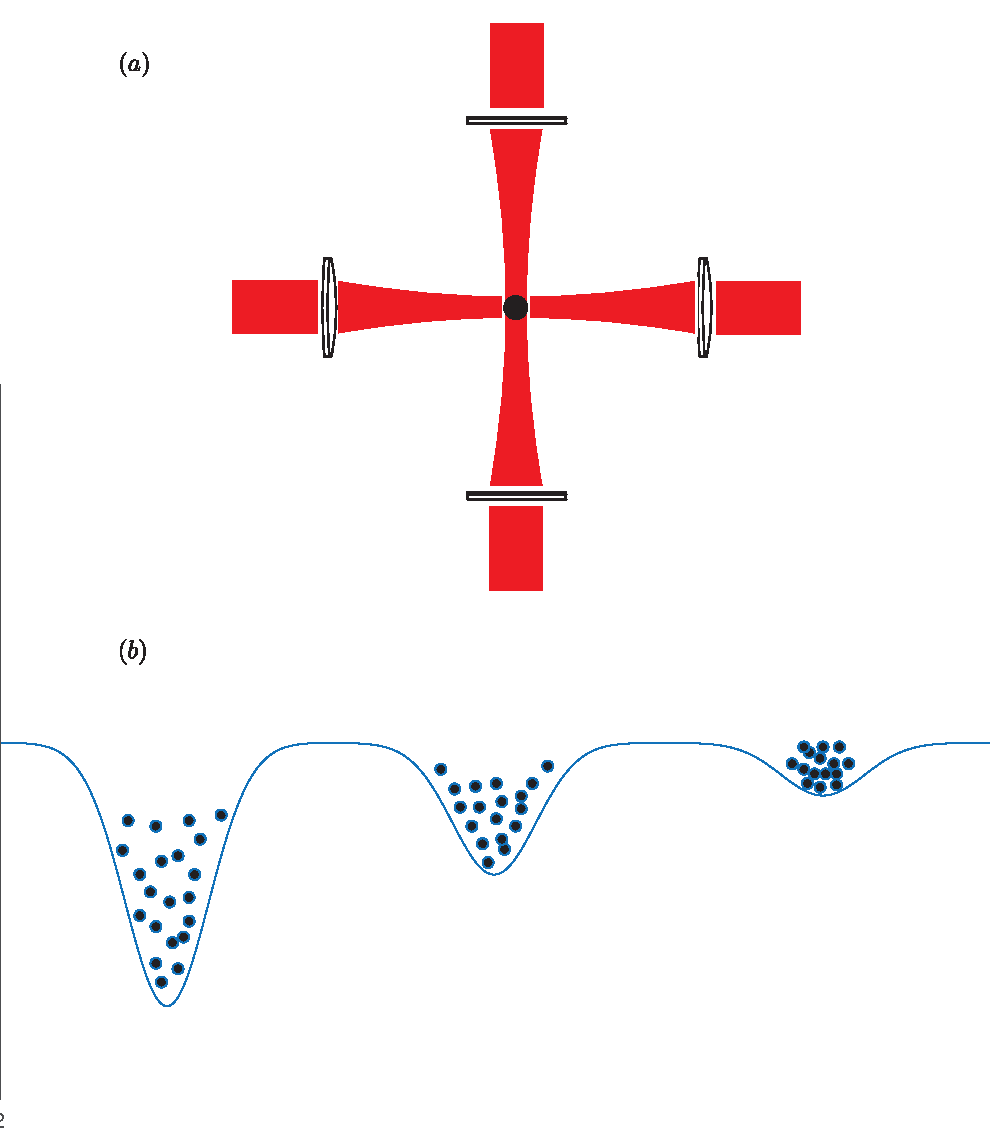
\includegraphics[width=\textwidth]{Chapter2_secs/DipoleEvap.pdf}
    \caption{Dipole evaporation. (a) A sketch of crossed dipole trap formed by two red detuned laser beams. (b)Dipole evaporative cooling process. }
    \label{fig:DipoleEvap}
\end{figure}

Fig.~(\ref{fig:DipoleEvap})(a) shows a sketch of a crossed dipole trap which is widely used in cold atoms labs. A single Gaussian beam has a Gaussian intensity profile in its cross-sectional plane. Longitudinally, the width of the trapping potential is the Rayleigh length which is typically much larger than the beam width. So the confinement in the longitudinal direction is much weaker than it is in the cross-sectional directions. The crossed dipole trap solves this problem by adding the second dipole beam which provides confinement in the longitudinal direction of the first dipole beam.

Fig.~(\ref{fig:DipoleEvap})(b) shows the process of dipole evaporative cooling by continuously lowering the dipole trapping potential and allowing the high energy atoms to escape the trap and the rest of the atoms to thermalize to a lower temperature \cite{adams1995evaporative,lee1996raman}. In the escaping and rethermalizing process, the remaining atoms have much lower average energy and they tend to occupy a smaller volume at the center of the trap, thus increase the phase space density (\ref{phase space density}). 

